\documentclass[]{article}

\usepackage{tikz}
\usepackage{pgfplots}

%opening
\title{Concurrent Game of Life}
\author{
	Kai Hulme\\
	Computer Science\\
	\texttt{kh16747@my.bristol.ac.uk}
	\and
	Jack Bond-Preston\\
	Computer Science\\
	\texttt{jb17662@my.bristol.ac.uk}
}
\date{December 2018}

\begin{document}

\maketitle
\clearpage

\section{Functionality and Design}

...

\clearpage

\section {Tests and Experiments}

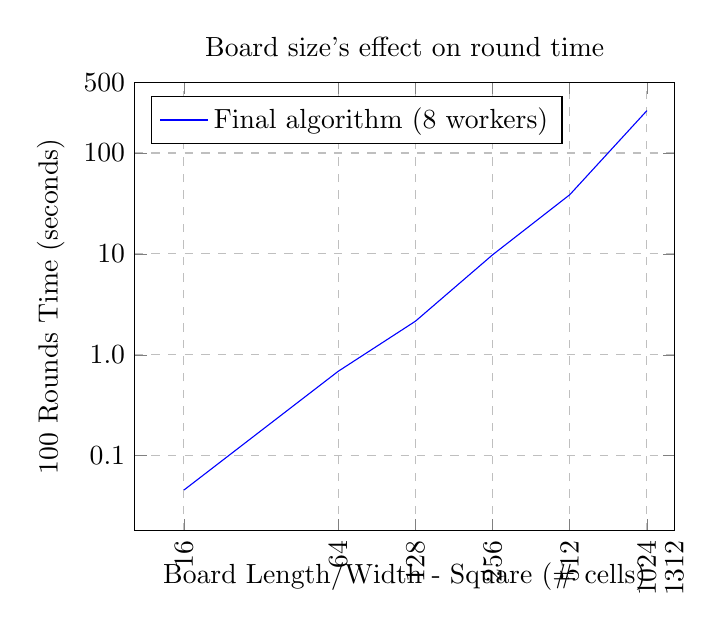
\begin{tikzpicture}
\begin{axis}[
	title={Board size's effect on round time},
	xlabel={Board Length/Width - Square (\# cells)},
	ylabel={100 Rounds Time (seconds)},
	xmin=0, xmax=1312,
	ymin=0, ymax=500,
	xtick={16, 64, 128, 256, 512, 1024, 1312},
	xticklabels={16, 64, 128, 256, 512, 1024, 1312},
	x tick label style={rotate=90, anchor=east},
	ytick={0.1, 1.0, 10, 100, 500},
	yticklabels={0.1, 1.0, 10, 100, 500},
	legend pos=north west,
	grid style=dashed,
	ymode=log,
	xmode=log,
	log basis x=2,
	grid=both,
	xlabel style={
		at={(0.5, -0.05)}
	}
]

% 8 workers skipping dead areas
\addplot[
	color=blue
]
coordinates {
	(16, 0.045632)
	(64, 0.686599)
	(128, 2.15193)
	(256, 9.795099)
	(512, 38.607723)
	(1024, 263.114624)
};

\legend{
	Final algorithm (8 workers)
}

\end{axis}
\end{tikzpicture}

\begin{tikzpicture}
\begin{axis}[
	title={Optimisation speedups},
	xtick=data,
	ylabel={Speed ($ = \frac{100}{time}$) Increase from Original Algorithm (\%)},
	xlabel={Board Length/Width - Square (\# cells)},
	legend style={
		at={(0.5, -0.15)},
		anchor=north,
		legend columns=2,
		/tikz/every even column/.append style={column sep=0.5cm}
	},
	ybar,
	symbolic x coords={16, 64, 128, 256, 512, 1024, 1312},
	bar width=7,
	width=12cm,
	ymajorgrids,
	legend cell align=left
]

\addplot
coordinates {
	(16, 15)
	(64, 13)
	(128, 13)
	(256, 15)
	(512, 8)
	(1024, 8)
	(1312, 5)
};

\addplot
coordinates {
	(16, 66)
	(64, 66)
	(128, 112)
	(256, 85)
	(512, 88)
	(1024, 10)
	(1312, 15)
};

\addplot
coordinates {
	(16, -3)
	(64, -9)
	(128, 12)
	(256, 4)
	(512, 12)
	(1024, -16)
	(1312, -12)
};

\addplot
coordinates {
	(16, 2)
	(64, -8)
	(128, 19)
	(256, 39)
	(512, 50)
	(1024, -14)
	(1312, -10)
};

\legend{
	8 Worker Less Checks,
	8 Worker Fully Optimised,
	4 Worker Normal Channels,
	4 Worker Streaming Channels
}
\end{axis}
\end{tikzpicture}

\clearpage

\section {Critical Analysis}

...

\end{document}
